      \let\negmedspace\undefined
\let\negthickspace\undefined
\documentclass[journal]{IEEEtran}
\usepackage[a5paper, margin=10mm, onecolumn]{geometry}
\usepackage{lmodern} 
\usepackage{tfrupee} 

\setlength{\headheight}{1cm} % Set the height of the header box
\setlength{\headsep}{0mm}     % Set the distance between the header box and the top of the text

\usepackage{gvv-book}
\usepackage{gvv}
\usepackage{cite}
\usepackage{amsmath,amssymb,amsfonts,amsthm}
\usepackage{algorithmic}
\usepackage{graphicx}
\usepackage{textcomp}
\usepackage{xcolor}
\usepackage{txfonts}
\usepackage{listings}
\usepackage{enumitem}
\usepackage{mathtools}
\usepackage{gensymb}
\usepackage{comment}
\usepackage[breaklinks=true]{hyperref}
\usepackage{tkz-euclide} 
\usepackage{listings}                                      
\def\inputGnumericTable{}                                 
\usepackage[latin1]{inputenc}                                
\usepackage{color}                                            
\usepackage{array}                                            
\usepackage{longtable}
\usepackage{multicol}
\usepackage{calc}                                             
\usepackage{multirow}                                         
\usepackage{hhline}                                           
\usepackage{ifthen}                                           
\usepackage{lscape}
\begin{document}

\bibliographystyle{IEEEtran}
\vspace{3cm}

\title{4.3.20}
\author {EE25BTECH11031 - Sai Sreevallabh}
% \maketitle
% \newpage
% \bigskip
{\let\newpage\relax\maketitle}

\renewcommand{\thefigure}{\theenumi}
\renewcommand{\thetable}{\theenumi}
\setlength{\intextsep}{10pt} % Space between text and floats


\numberwithin{equation}{enumi}
\numberwithin{figure}{enumi}
\renewcommand{\thetable}{\theenumi}

\textbf{Question: }\\

Find the area of the triangle $\triangle ABC$ bounded by the lines $4x-y+5 = 0$, $x+y-5 = 0$ and $x-4y+5 = 0$. \\

\textbf{Solution: }\\

Given lines can be written as: 

\begin{align}
    \myvec{4&-1}\myvec{x\\y} = -5 \label{eq:1}
\end{align}

\begin{align}
    \myvec{1&1}\myvec{x\\y} = 5 \label{eq:2}
\end{align}

\begin{align}
    \myvec{1&-4}\myvec{x\\y} = -5 \label{eq:3}
\end{align}

Solving equations \eqref{eq:1} and \eqref{eq:2} to get the point of intersection $\vec{A}$:

\begin{align}
    \myvec{1&1\\4&-1}\myvec{x\\y} =& \myvec{5\\-5}
\end{align}

Making the Augmented Matrix and converting to echelon form

\begin{align}
    \augvec{2}{1}{1&1&5\\4&-1&-5} \xleftrightarrow[]{R_2 \xrightarrow{} R_2-4R_1} \augvec{2}{1}{1&1&5\\0&-5&-25}
\end{align}

We get
\begin{align}
    \vec{A}=\myvec{0\\5}
\end{align}

Solving equations \eqref{eq:2} and \eqref{eq:3} to get the point of intersection $\vec{B}$

\begin{align}
    \augvec{2}{1}{1&1&5\\1&-4&-5} \xleftrightarrow[]{R_2 \xrightarrow{} R_2-R_1} \augvec{2}{1}{1&1&5\\0&-5&-10}
\end{align}

We get
\begin{align}
    \vec{B}= \myvec{3\\2}
\end{align}

Solving equations \eqref{eq:1} and \eqref{eq:3} to get the point of intersection $\vec{C}$

\begin{align}
    \augvec{2}{1}{1&-4&-5\\4&-1&5} \xleftrightarrow[]{R_2 \xrightarrow{} R_2-4R_1} \augvec{2}{1}{1&-4&-5\\0&15&15}
\end{align}

We get
\begin{align}
    \vec{C}= \myvec{-1\\1}
\end{align}

The vertices of the triangle are

\begin{align}
    \vec{A}=\myvec{0\\5} \ ,\ \vec{B}= \myvec{3\\2} \ , \ \vec{C}= \myvec{-1\\1}
\end{align}

Now

\begin{align}
    \vec{B-A} = \myvec{3\\-3} \ \text{and} \ \vec{C-A} = \myvec{-1\\-4}
\end{align}\\

Area of the triangle $\triangle ABC$ is given by
\begin{align}
    \frac{1}{2}\norm{\brak{\vec{B-A}}\times\brak{\vec{C-A}}}
\end{align}

\begin{align}
    =&\ \ \frac{1}{2}\norm{\myvec{3\\-3}\times\myvec{-1\\-4}}\\
    =&\ \ \frac{15}{2}
\end{align}

Hence,
\begin{align}
    ar\brak{\triangle ABC} = \frac{15}{2}
\end{align}\\

$\therefore$ The area of the triangle formed by the given three lines is $\frac{15}{2}$ units. 

\begin{figure}[H]
    \centering
    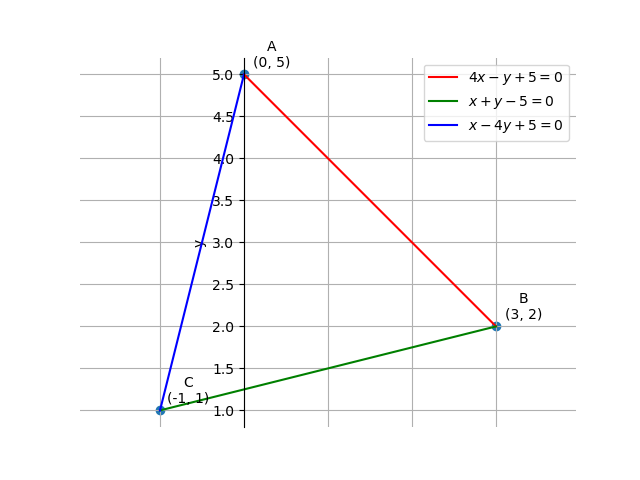
\includegraphics[width=1\columnwidth]{Figs/plot(py).png}
\end{figure}

\end{document}
